%!TEX root = ..\..\dissertation.tex
\section{Challenges in Manufacturing System Platform Development}\label{sec:challenges}
\cref{paper:APMS2018} is entitled \citetitle{SorensenAPMS2018}, written for and presented at the 2018 conference on Advances in Production Management Systems (APMS2018).
It relates to and addresses \cref{resq3} by answering the following sub-question:
\begin{enumerate}[leftmargin=3em, label=RQ3.\arabic*]
    \item Which challenges do mature manufacturers face over time, when developing manufacturing system platforms?
\end{enumerate}
The study documented in \cref{paper:APMS2018} was carried out with a design science research approach through an evolving case study with the industrial collaborator.
Its purpose was to sum up and outline the challenges encountered during three years of manufacturing system platform development projects with the industry.
This was done to set the stage for research into areas of manufacturing system platform development benefitting manufacturers, and advancing the field as a whole.

\subsection{Extended Abstract}
\subsubsection*{Introduction \& Method}
Incorporating changeability into manufacturing systems appears to be a logical choice to managing variety in products~\parencite{HodaC,ElMaraghy2013629}
However, achieving this remains a difficult process despite research into platforms, \gls{glos:codev}~\parencite{MichaelisJohannesson}, and co-platforming~\parencite{ElMaraghy2015407} paving the way for using manufacturing system platforms during manufacturing system design~\parencite{BossenPbCd,Andersen2017179}.
With these collaborative approaches and integrated modelling gaining traction~\parencite{Michaelis2015203,LANDAHL201661}, the need for co-existing product and manufacturing system \gls{glos:platform}s seems clear.
To highlight these challenges, and frame them for future research, this study presents a number of challenges, lessons, and experiences on development of manufacturing systems, based on an evolving case study spanning four projects and three years.

The evolving case study is structured based on the framework for design science research in information systems by \textcite{10.2307/25148625}.
This framework is focused on developing new \gls{glos:artefact}s, new theories, and making new experiences, applying them all in an appropriate environment, and recording them in a knowledge base.
The knowledge base itself essentially acts as a platform, as resources can be pulled from it and applied to a specific context, with the results being used to update the knowledge base, making it more comprehensive.
Artefacts are used to communicate, represent, and solve problems (construct, model, and method artefacts respectively) as well as demonstrating the feasibility of both artefacts and solutions (instantiations).
They can be considered somewhat analogous to the concepts of \gls{glos:viewp}s (constructs and methods) and \gls{glos:view}s (models and instantiations) from software architecture~\parencite{ISO42010}.

\subsubsection*{The Case}
For the evolving case study, the case company is a large Danish manufacturer of discrete consumer and OEM products.
The case study covers a number of different factories and systems both in Denmark and other countries, manufacturing both mechatronic and purely mechanical components and products.
As the case study evolved, the scope was gradually changed to reflect the progress of development and the number of participants, as well as considering the timing of parallel projects and the company's internal roadmaps.
As the knowledge base on manufacturing system platforms was somewhat limited prior to initiation of the evolving case study, applicable theories and \gls{glos:artefact}s from software architecture and product platforms were employed.
The application environment for new artefacts and theories was provided by the case study environment, including the people, organisations, and technologies relevant to the case company.

\subsubsection*{Results}
The evolving case study consists of four sequential projects, each with their own purpose, scope, and group of participants.
An overview of the four projects is shown on \cref{fig:evoCase}.
\begin{figure}[tb]
  \centering
  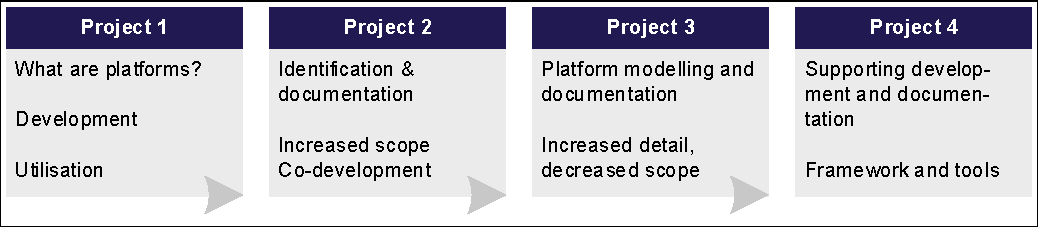
\includegraphics[width=.9\textwidth, trim= 2 4 2 2, clip]{mainmatter/researchResults/figures/evoCase.pdf}
  \caption[The four projects in the evolving case study.]
  {The four projects in the evolving case study.
  Adapted from~\parencite{SorensenAPMS2018}.}\label{fig:evoCase}
\end{figure}
Certain challenges appeared throughout the four projects; some repeatedly, while others were unique to the specific project.
All of them are outlined in the following.

One challenge was prevalent during all four projects, but was especially an issue during the first project.
This was the focus on product platforms in literature and the general lack of research on manufacturing system platforms.
Knowledge on platforms among the participants of the project was sparse, so questions related to the nature and utilisation of platforms dominated the project.
The ambition for initiating the platform projects was to design an \gls{glos:RMS} which, through platforms, achieved an improved level of utilisation and robustness.
Because of this, there was also a need for clarifying the connection between \gls{glos:RMS}, \gls{glos:changeability}, and platforms.
Five manufacturing systems in the same production segment, producing five product variants within the same product family, were scoped for the first project.
Based on these five systems and product variants, a first iteration of an extractive platform development approach was created to show platforms could be developed based on existing manufacturing systems, and, through a workshop, how the platform could be used to design an \gls{glos:RMS} and its various configurations for the company.

For the second project, the scope was increased to cover 23 manufacturing systems and 25 corresponding product architectures.
With this, both the scope and number of project participants increased greatly. 
Here, alignment of participant knowledge on both platforms and project purpose was key; especially with participants coming from multiple departments within the company, each with their own specific goals for participation.
The focus for this project was on making knowledge on platforms more accessible throughout the company, by identifying, developing, and documenting potential platforms, thereby creating concrete examples of manufacturing system platforms that could be communicated in the various departments.
It was also an attempt at breaking down the ``silos'' in which individual departments isolate themselves.
Overall, the project was carried out according to the Four Loops of Concern (FLC) as outlined in \parencite{SorensenMCPC2017}.
As such, the project was an evaluation of the FLC, both its vocabulary and its use as a platform development method. 
Several model and instantiation artefacts were created during the project using \eg{} function-means trees, generic organ diagrams, interface diagrams, radar diagrams, technical drawings, \etc. 
Finally, the project resulted in the creation of an initial format for documenting product and manufacturing system platforms.

In the third project, the scope was drastically decreased to focus on a single key process carried out by all 23 manufacturing systems covered in the second project.
The intention for this project was to increase the level of detail while continuing work on a documentation format or system for platforms, as the documentation system prior to the third project was still reliant on individual text documents, static figures, and tables.
To better accommodate individual stakeholder concerns, a back end model for generating customised documentation containing only the requested information was developed.
The intention was to have all available information on a given platform collected in one model, and then generate documentation specifically for various stakeholders in order to avoid information overload.
Using a modelling formalism was also intended to promote consistency in terms of how platforms were described, documented, and communicated.
It was based on the configurable component framework (CCF) because of its integration of both product and manufacturing system platforms \parencite{Claesson2006,Michaelis2015203}.
The selected process was documented as a platform, with all current and planned future configurations documented as configurable components with interactions, interfaces, constraints, requirements, and design solutions.

The fourth project is, at the time of writing, still on-going.
Its purpose is to create a comprehensive platform framework supporting the development, documentation, and utilisation of manufacturing system platforms.
The framework itself will be based around the conceptual model by \textcite{BossenCMod} and the ISO 42010 standard on architecture descriptions~\parencite{ISO42010}, thus employing concepts, tools, and methods from software architecture and systems engineering.
This is further an attempt at addressing both the lack of research on manufacturing system platforms, as well as the lack of concrete tools assisting manufacturers in their platform development process.
\posscite{SorensenCMS2018} classification scheme is one concrete part of this framework, which, along side a manufacturing system classification code, is intended to help manufacturers structure and standardise their information and data collection on existing manufacturing systems, so these systems can form the base for development of new platforms.

\subsubsection*{Conclusions}
As the case company progressed through the four projects outlined above, all participants' knowledge on \gls{glos:platform}s grew significantly.
A multitude of approaches and tools were tested under a variety of circumstances and project scopes.
The main challenges encountered during this evolving case study can be summarised as follows:
\begin{itemize}
  \item Little to no consistency and coherency in vocabulary and development process.
  \item Participant knowledge on platforms and project scope was not aligned.
  \item Frequent miscommunication between departments in the case company.
  \item Very few available examples of platform documentation.
  \item Minimal available research and tools for manufacturing system platforms.
\end{itemize}

\subsection{Implications}
In concretising several challenges on manufacturing system platforms and particularly their development and documentation, the paper outlined above sets the stage for research on addressing these challenges and concerns.
Particularly the vocabulary proved inconsistent and problematic as scope and project participants changed.
This, coupled with a persistent need to collect more information on existing manufacturing systems, calls for a structured approach and tool if platforms are to be developed based on existing systems.
The outcome is summarised as:
\begin{enumerate}
  \item A list of frequent challenges related to manufacturing system development.
  \item Suggestions on how to address these frequent challenges.
  \item Sets the stage for research on concrete tools for manufacturing system platform development.
  \item Feeds back experiences to the knowledge base on manufacturing system platforms.
\end{enumerate}